\chapter{Конструкторская часть}

В данном разделе будут приведены схемы алгоритмов нахождения расстояний Левенштейна и Дамерау-Левенштейна, приведены описание используемых типов данных, оценки памяти, а также описана структура программного обеспечения.

\section{Требования к программному обеспечению}\label{section:requirements}

К программе предъявлен ряд функциональных требований: входные данные --- две строки, выходные данные --- результат работы всех алгоритмов поиска расстояний, целое число.

Кроме того, программа должна соответствовать следующим требованиям:
\begin{itemize}[label=---]
	\item наличие интерфейса для выбора действий;
	\item должна обрабатывать строки;
	\item возможность обработки строк, включающих буквы как на латинице, так и на кириллице;
	\item наличие функциональности замера процессорного времени работы реализаций алгоритмов поиска расстояний Левенштейна и Дамерау-Левен- штейна.
\end{itemize}

\section{Разработка алгоритмов}

На вход алгоритмов подаются строки $S_1$ и $S_2$.

На рисунках \ref{fig:Liter1} -- \ref{fig:Liter2} представлены схемы алгоритма поиска расстояния Левенштейна.
На рисунках \ref{fig:DLiter1} -- \ref{fig:DLrechash2} представлены схемы алгоритмов поиска расстояния Дамерау-Левенштейна.

\begin{figure}[h]
	\centering
	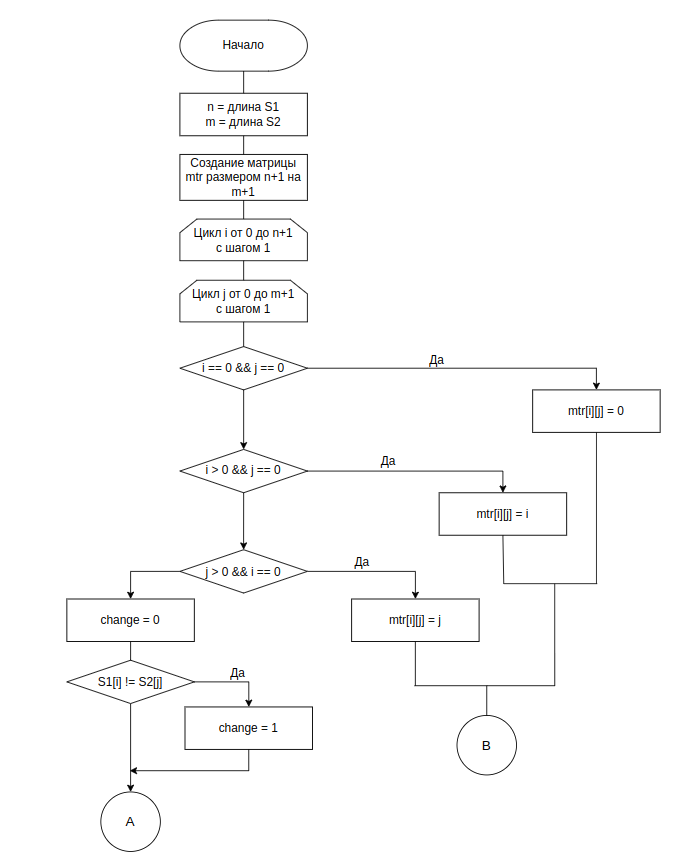
\includegraphics[width=\textwidth]{img/levmatr1.png}
	\caption{Схема 1 нерекурсивного алгоритма нахождения расстояния Левенштейна}
	\label{fig:Liter1}
\end{figure}

\clearpage

\begin{figure}[h]
	\centering
	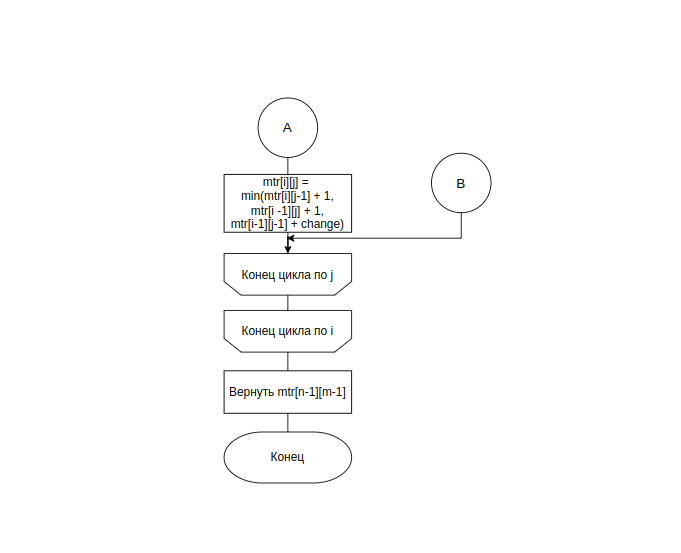
\includegraphics[width=\textwidth]{img/levmatr2.png}
	\caption{Схема 2 нерекурсивного алгоритма нахождения расстояния Левенштейна}
	\label{fig:Liter2}
\end{figure}

\clearpage

\begin{figure}[h]
	\centering
	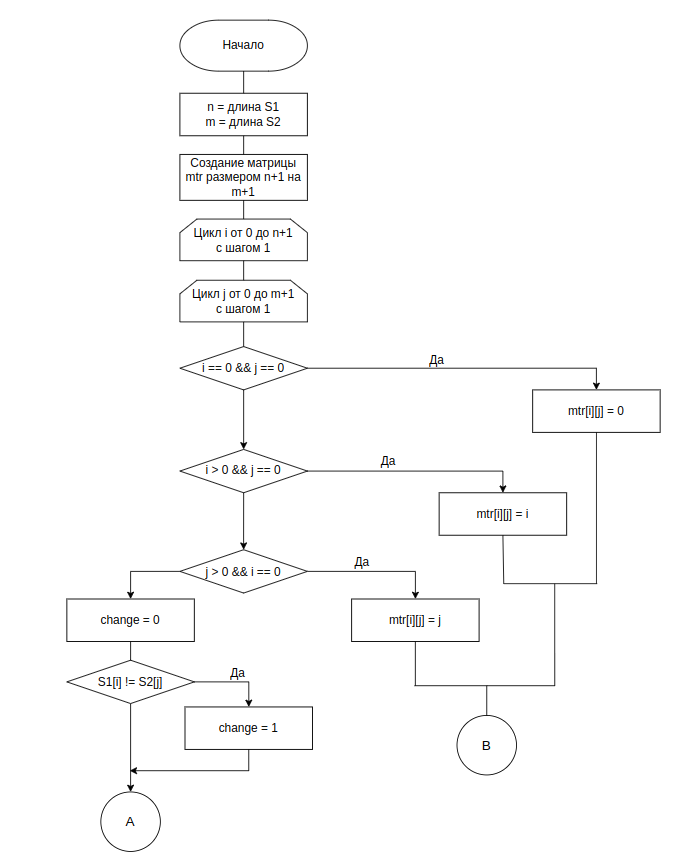
\includegraphics[width=\textwidth]{img/dliter1.png}
	\caption{Схема 1 нерекурсивного алгоритма нахождения расстояния Дамерау-Левенштейна}
	\label{fig:DLiter1}
\end{figure}

\clearpage

\begin{figure}[h]
	\centering
	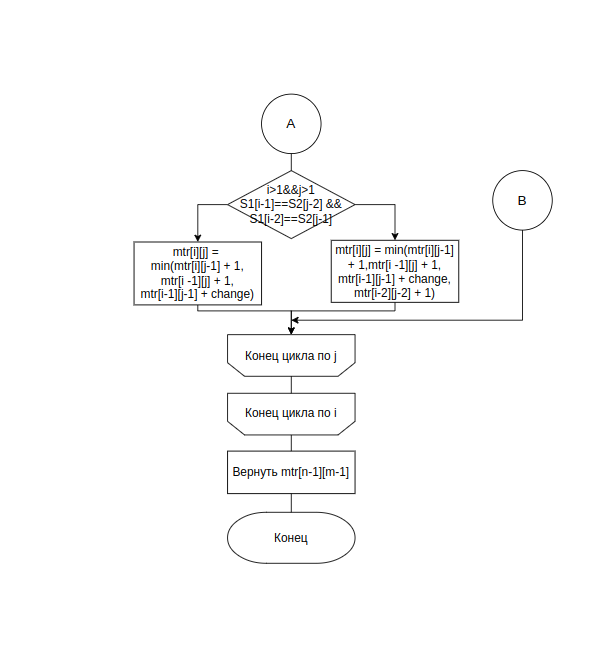
\includegraphics[width=\textwidth]{img/dliter2.png}
	\caption{Схема 2 нерекурсивного алгоритма нахождения расстояния Дамерау-Левенштейна}
	\label{fig:DLiter2}
\end{figure}

\clearpage

\begin{figure}[h]
	\centering
	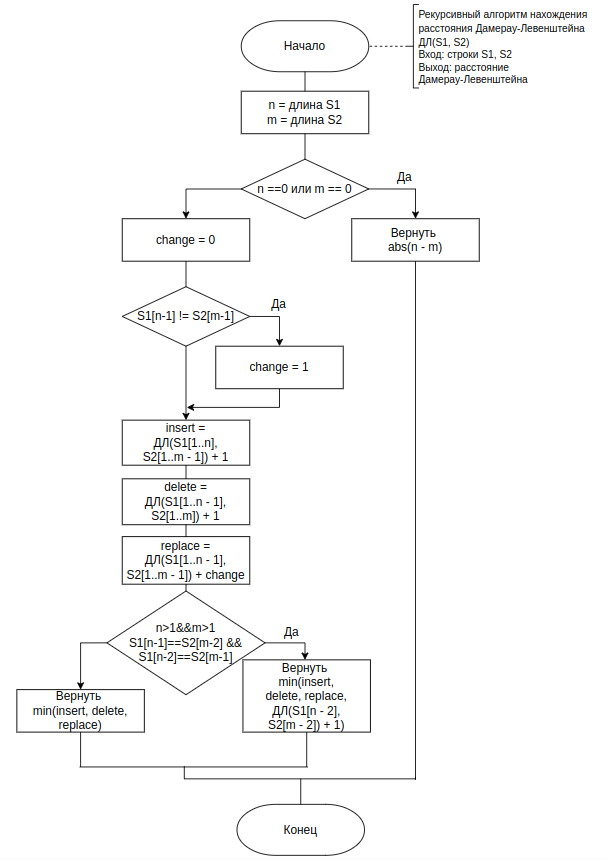
\includegraphics[width=\textwidth]{img/dlrec.png}
	\caption{Схема рекурсивного алгоритма нахождения расстояния Дамерау-Левенштейна}
	\label{fig:DLrec}
\end{figure}

\clearpage

\begin{figure}[h]
	\centering
	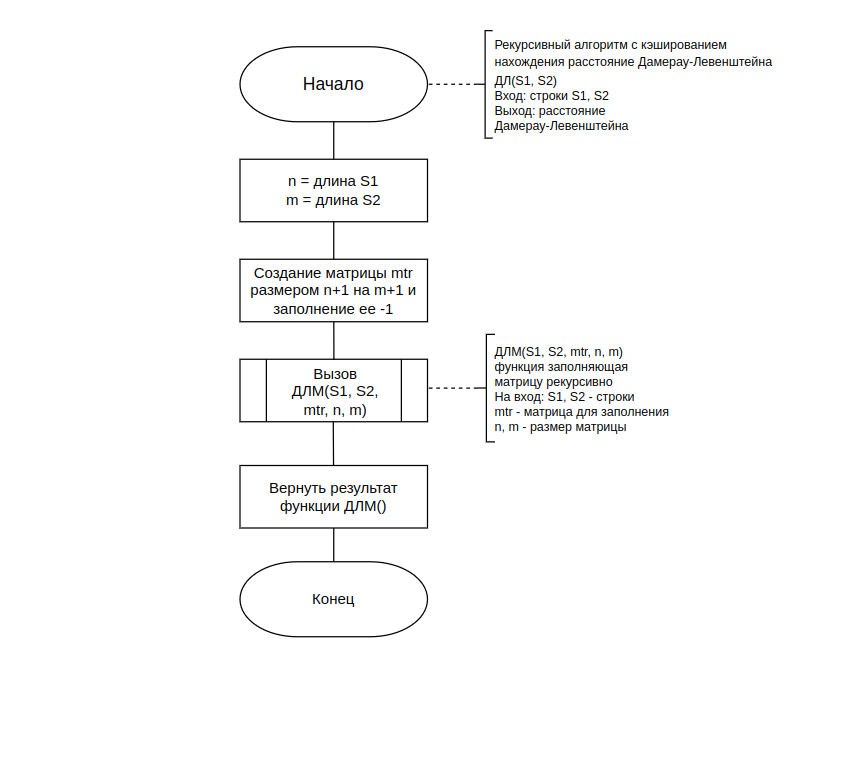
\includegraphics[width=\textwidth]{img/dlrechash1.png}
	\caption{Схема 1 рекурсивного алгоритма нахождения расстояния Дамерау-Левенштейна с кешированием}
	\label{fig:DLrechash1}
\end{figure}

\clearpage

\begin{figure}[h]
	\centering
	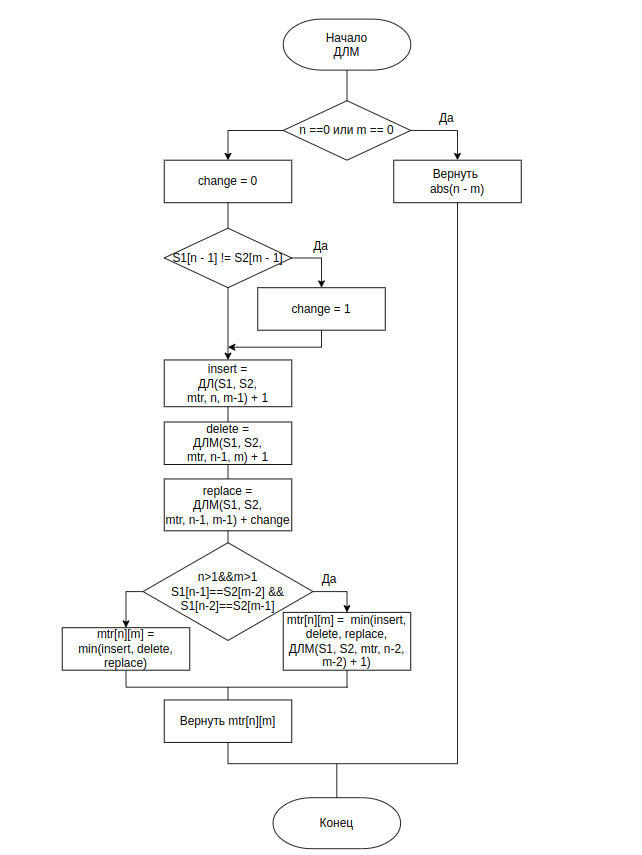
\includegraphics[width=\textwidth]{img/dlrechash2.png}
	\caption{Схема 2 рекурсивного алгоритма нахождения расстояния Дамерау-Левенштейна с кешированием}
	\label{fig:DLrechash2}
\end{figure}

\clearpage

\section{Описание используемых типов данных}

При реализации алгоритмов будут использованы следующие структуры данных:

\begin{itemize}
	\item строка --- массив типа $wchar$ размером длины строки;
	\item матрица --- двумерный массив значений типа $int$.
\end{itemize}

\section*{Вывод}

В данном разделе на основе теоретических данных были построены схемы
требуемых алгоритмов, выбраны используемые типы данных.
